\documentclass[aspectratio=169, 10pt]{beamer}

% ============================================================
% THEME & COLORS - Madrid Standard
% ============================================================
\usetheme{Madrid}
\usecolortheme{default} % Standard Blue Madrid look
\setbeamertemplate{navigation symbols}{} % Remove nav symbols for cleaner look
\setbeamertemplate{blocks}[rounded][shadow=true]

% Custom Colors (Kept for Diagrams)
\definecolor{espblue}{RGB}{0, 100, 148}
\definecolor{espgold}{RGB}{255, 196, 37}
\definecolor{codegreen}{RGB}{40, 167, 69}
\definecolor{codeorange}{RGB}{253, 126, 20}
\definecolor{codepurple}{RGB}{111, 66, 193}
\definecolor{codered}{RGB}{220, 53, 69}
\definecolor{darkbg}{RGB}{40, 44, 52}
\definecolor{lightgray}{RGB}{248, 249, 250}
\definecolor{appred}{RGB}{239, 154, 154}
\definecolor{appblue}{RGB}{144, 202, 249}
\definecolor{apppurple}{RGB}{206, 147, 216}
\definecolor{osgreen}{RGB}{165, 214, 167}
\definecolor{kernelblue}{RGB}{100, 181, 246}
\definecolor{hwgray}{RGB}{189, 189, 189}

% ============================================================
% PACKAGES
% ============================================================
\usepackage{tikz}
\usetikzlibrary{shapes.geometric, shapes.symbols, shapes.misc, arrows.meta, positioning, calc, fit, backgrounds, decorations.pathreplacing, shadows, patterns, chains, matrix}
\usepackage{listings}
\usepackage{xcolor}
\usepackage{amsmath, amssymb}
\usepackage{booktabs}
\usepackage{graphicx}

% ============================================================
% CODE LISTING STYLES
% ============================================================
\lstdefinestyle{cstyle}{
    language=C,
    basicstyle=\ttfamily\tiny,
    keywordstyle=\color{codepurple}\bfseries,
    stringstyle=\color{codegreen},
    commentstyle=\color{gray}\itshape,
    numberstyle=\tiny\color{gray},
    breaklines=true,
    showstringspaces=false,
    tabsize=2,
    frame=single,
    backgroundcolor=\color{lightgray},
    morekeywords={uint32_t, int32_t, size_t, Elf32_Phdr, esp_err_t, bool, ssize_t},
    escapeinside={(*@}{@*)},
}

\lstnewenvironment{ccode}[1][]
{\lstset{style=cstyle,title={\tiny #1}}}
{}

% ============================================================
% TikZ STYLES
% ============================================================
\tikzset{
    layerbox/.style={draw, rectangle, minimum width=2.5cm, minimum height=0.7cm, font=\scriptsize, align=center, thick},
    appbox/.style={layerbox, fill=appred!60},
    osbox/.style={layerbox, fill=osgreen!60},
    kernelbox/.style={layerbox, fill=kernelblue!60},
    hwbox/.style={layerbox, fill=hwgray!60},
    shimbox/.style={layerbox, fill=espgold!40},
    guestbox/.style={layerbox, fill=codegreen!30, draw=codegreen!70!black},
    component/.style={draw, rectangle, rounded corners=2pt, minimum width=2.2cm, minimum height=0.6cm, font=\scriptsize, align=center},
    kernel/.style={component, fill=espblue!20, draw=espblue},
    guest/.style={component, fill=codegreen!20, draw=codegreen!70!black},
    hardware/.style={component, fill=gray!30, draw=gray!60},
    shim/.style={component, fill=espgold!30, draw=espgold!70!black},
    danger/.style={component, fill=codered!20, draw=codered},
    dataarrow/.style={-{Stealth[length=2mm]}, thick, draw=espblue},
    callarrow/.style={-{Stealth[length=2mm]}, thick, draw=codegreen!70!black},
    annotation/.style={font=\tiny\itshape, text=gray},
}

% ============================================================
% METADATA
% ============================================================
\title[ESP32 Thin Linux]{ESP32 Thin Linux Compatibility Layer}
\subtitle{A Unikernel Approach to Dynamic ELF Execution on No-MMU Hardware}
\author[Joshi \& Sabat]{Dhruv Joshi (2022EE32079) \and Gourab Raj Sabat (2022EE11675)}
\institute[IIT Delhi]{Department of Electrical Engineering \\ Indian Institute of Technology Delhi}
\date{BTP Fall 2025 \\ Supervisor: Prof. Kaushik Saha}

\begin{document}

% ============================================================
% TITLE SLIDE
% ============================================================
\begin{frame}
\titlepage
\end{frame}

% ============================================================
% THE DESIGN PROBLEM
% ============================================================
\begin{frame}{The Design Problem}
    \textbf{Goal:} Execute standard POSIX C applications on ESP32 \textit{without reflashing firmware}.

    \vspace{0.2cm}
    \begin{columns}[T]
        \column{0.48\textwidth}
        \begin{block}{Why is this hard?}
            \begin{itemize}
                \item ESP32 has \textbf{no MMU} --- no virtual memory
                \item Firmware is \textbf{statically linked}
                \item 50-line app change $\to$ reflash 4MB
                \item No dynamic linker (\texttt{ld.so})
            \end{itemize}
        \end{block}

        \column{0.48\textwidth}
        \begin{block}{Approach: Library OS}
            \begin{itemize}
                \item Linux \textit{API} without Linux \textit{architecture}
                \item Runtime ELF loading + symbol resolution
                \item Syscall translation layer (shims)
                \item Unix-style \texttt{/dev/} abstraction
            \end{itemize}
        \end{block}
    \end{columns}

    \vspace{0.3cm}
    \begin{alertblock}{Result}
        \centering
        Standard C applications run \textit{unmodified}, loaded at runtime over WiFi.
    \end{alertblock}
\end{frame}

% ------------------------------------------------------------
\begin{frame}{Where TLCL Fits: OS Architecture Taxonomy}
    \begin{center}
        % Scaling diagram to fit slide
        \resizebox{0.95\textwidth}{!}{
            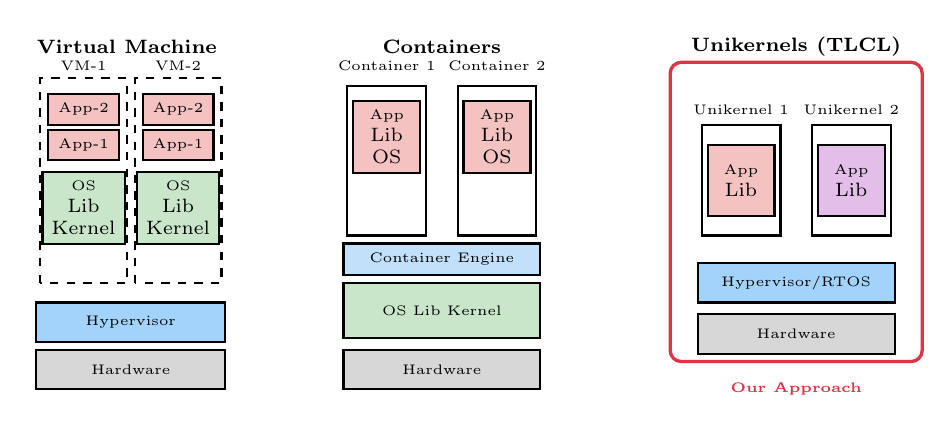
\begin{tikzpicture}
                % === VM ===
                \node[font=\scriptsize\bfseries] at (0, 4.2) {Virtual Machine};
                
                % VM-1 dashed box
                \draw[dashed, thick] (-1.1, 1.2) rectangle (0, 3.8);
                \node[font=\tiny] at (-0.55, 3.95) {VM-1};
                \node[appbox, minimum width=0.9cm, minimum height=0.35cm] at (-0.55, 3.4) {\tiny App-2};
                \node[appbox, minimum width=0.9cm, minimum height=0.35cm] at (-0.55, 2.95) {\tiny App-1};
                \node[osbox, minimum width=0.9cm, minimum height=0.7cm] at (-0.55, 2.15) {\tiny OS\\Lib\\Kernel};
                
                % VM-2 dashed box
                \draw[dashed, thick] (0.1, 1.2) rectangle (1.2, 3.8);
                \node[font=\tiny] at (0.65, 3.95) {VM-2};
                \node[appbox, minimum width=0.9cm, minimum height=0.35cm] at (0.65, 3.4) {\tiny App-2};
                \node[appbox, minimum width=0.9cm, minimum height=0.35cm] at (0.65, 2.95) {\tiny App-1};
                \node[osbox, minimum width=0.9cm, minimum height=0.7cm] at (0.65, 2.15) {\tiny OS\\Lib\\Kernel};
                
                \node[kernelbox, minimum width=2.4cm, minimum height=0.5cm] at (0.05, 0.7) {\tiny Hypervisor};
                \node[hwbox, minimum width=2.4cm, minimum height=0.5cm] at (0.05, 0.1) {\tiny Hardware};
                
                % === Containers ===
                \node[font=\scriptsize\bfseries] at (4, 4.2) {Containers};
                
                \node[font=\tiny] at (3.3, 3.95) {Container 1};
                \node[font=\tiny] at (4.7, 3.95) {Container 2};
                
                \draw[thick] (2.8, 1.8) rectangle (3.8, 3.7);
                \node[appbox, minimum width=0.85cm, minimum height=0.9cm] at (3.3, 3.05) {\tiny App\\Lib\\OS};
                
                \draw[thick] (4.2, 1.8) rectangle (5.2, 3.7);
                \node[appbox, minimum width=0.85cm, minimum height=0.9cm] at (4.7, 3.05) {\tiny App\\Lib\\OS};
                
                \node[kernelbox, fill=kernelblue!40, minimum width=2.5cm, minimum height=0.4cm] at (4, 1.5) {\tiny Container Engine};
                \node[osbox, minimum width=2.5cm, minimum height=0.7cm] at (4, 0.85) {\tiny OS Lib Kernel};
                \node[hwbox, minimum width=2.5cm, minimum height=0.5cm] at (4, 0.1) {\tiny Hardware};
                
                % === Unikernels (TLCL) ===
                \node[font=\scriptsize\bfseries] at (8.5, 4.2) {Unikernels (TLCL)};
                
                \node[font=\tiny] at (7.8, 3.4) {Unikernel 1};
                \node[font=\tiny] at (9.2, 3.4) {Unikernel 2};
                
                \draw[thick] (7.3, 1.8) rectangle (8.3, 3.2);
                \node[appbox, minimum width=0.85cm, minimum height=0.9cm] at (7.8, 2.5) {\tiny App\\Lib};
                
                \draw[thick] (8.7, 1.8) rectangle (9.7, 3.2);
                \node[apppurple!60, minimum width=0.85cm, minimum height=0.9cm] at (9.2, 2.5) {};
                \node[appbox, fill=apppurple!60, minimum width=0.85cm, minimum height=0.9cm] at (9.2, 2.5) {\tiny App\\Lib};
                
                \node[kernelbox, minimum width=2.5cm, minimum height=0.5cm] at (8.5, 1.2) {\tiny Hypervisor/RTOS};
                \node[hwbox, minimum width=2.5cm, minimum height=0.5cm] at (8.5, 0.55) {\tiny Hardware};
                
                % Highlight TLCL
                \draw[very thick, codered, rounded corners] (6.9, 0.2) rectangle (10.1, 4.0);
                \node[font=\tiny\bfseries, text=codered] at (8.5, -0.15) {Our Approach};
            \end{tikzpicture}
        }
    \end{center}

    \vspace{0.1cm}
    \textbf{Key Insight:} TLCL links OS functionality \textit{into} the application runtime --- syscalls become function calls, not context switches.
\end{frame}

% ============================================================
% ARCHITECTURE OVERVIEW
% ============================================================
\begin{frame}{System Architecture Overview}
    \begin{center}
        \resizebox{0.95\textwidth}{!}{
            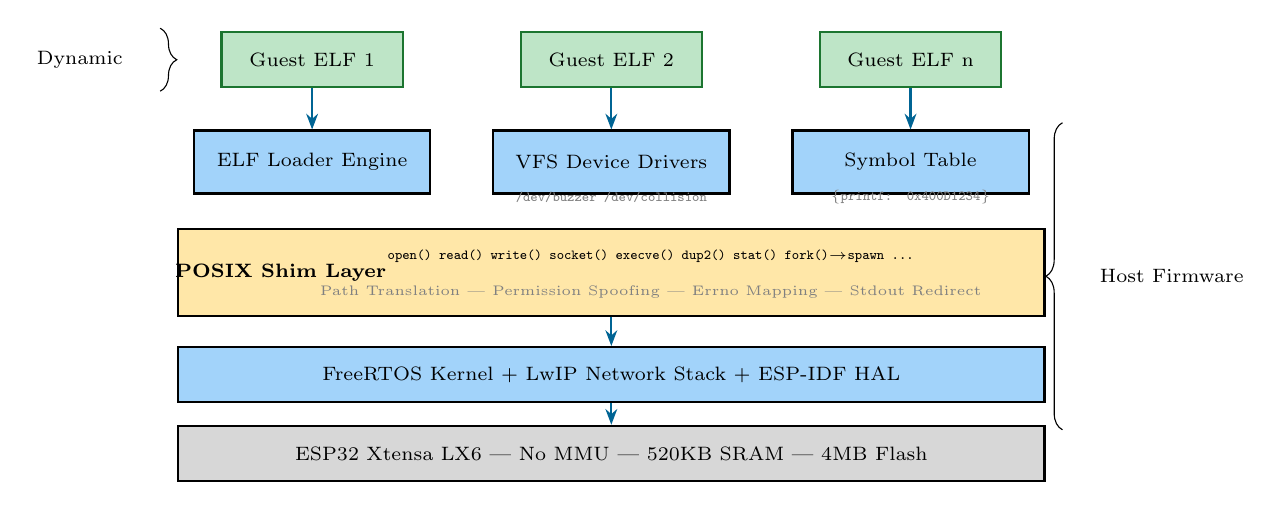
\begin{tikzpicture}
                % Hardware layer
                \node[hwbox, minimum width=11cm, minimum height=0.7cm] (hw) at (0,-0.4) 
                      {ESP32 Xtensa LX6 | No MMU | 520KB SRAM | 4MB Flash};
                
                % FreeRTOS layer
                \node[kernelbox, minimum width=11cm, minimum height=0.7cm] (rtos) at (0,0.6) 
                      {FreeRTOS Kernel + LwIP Network Stack + ESP-IDF HAL};
                
                % Shim layer
                \node[shimbox, minimum width=11cm, minimum height=1.1cm] (shim) at (0,1.9) {};
                \node[font=\scriptsize\bfseries] at (-4.2, 1.9) {POSIX Shim Layer};
                \node[font=\tiny, align=center] at (0.5, 2.1) 
                      {\texttt{open() read() write() socket() execve() dup2() stat() fork()$\to$spawn ...}};
                \node[font=\tiny, align=center, text=gray] at (0.5, 1.65) 
                      {Path Translation | Permission Spoofing | Errno Mapping | Stdout Redirect};
                
                % Middle components row
                \node[kernelbox, minimum width=3cm, minimum height=0.8cm] (loader) at (-3.8, 3.3) {ELF Loader Engine};
                
                \node[kernelbox, minimum width=3cm, minimum height=0.8cm] (vfs) at (0, 3.3) {VFS Device Drivers};
                \node[font=\tiny, text=gray] at (0, 2.85) {\texttt{/dev/buzzer  /dev/collision}};
                
                \node[kernelbox, minimum width=3cm, minimum height=0.8cm] (symtab) at (3.8, 3.3) {Symbol Table};
                \node[font=\tiny, text=gray] at (3.8, 2.85) {\texttt{\{printf: 0x400D1234\}}};
                
                % Guest Applications
                \node[guestbox, minimum width=2.3cm] (g1) at (-3.8, 4.6) {Guest ELF 1};
                \node[guestbox, minimum width=2.3cm] (g2) at (0, 4.6) {Guest ELF 2};
                \node[guestbox, minimum width=2.3cm] (g3) at (3.8, 4.6) {Guest ELF n};
                
                % Connections
                \draw[dataarrow] (g1) -- (loader);
                \draw[dataarrow] (g2) -- (vfs);
                \draw[dataarrow] (g3) -- (symtab);
                \draw[dataarrow] (shim) -- (rtos);
                \draw[dataarrow] (rtos) -- (hw);
                
                % Braces and labels
                \draw[decorate, decoration={brace, amplitude=6pt, raise=2pt}]
                      (5.8, -0.1) -- (5.8, 3.8) node[midway, right=8pt, font=\scriptsize] {Host Firmware};
                \draw[decorate, decoration={brace, amplitude=6pt, raise=2pt, mirror}]
                      (-5.8, 4.2) -- (-5.8, 5.0) node[midway, left=8pt, font=\scriptsize] {Dynamic};
            \end{tikzpicture}
        }
    \end{center}
\end{frame}

% ============================================================
% MEMORY ARCHITECTURE
% ============================================================
\begin{frame}{Memory Architecture: The No-MMU Constraint}
    \begin{columns}[T]
        \column{0.43\textwidth}
        \textbf{Harvard Architecture Split:}
        \vspace{0.2cm}
        \begin{center}
            \resizebox{0.9\textwidth}{!}{
                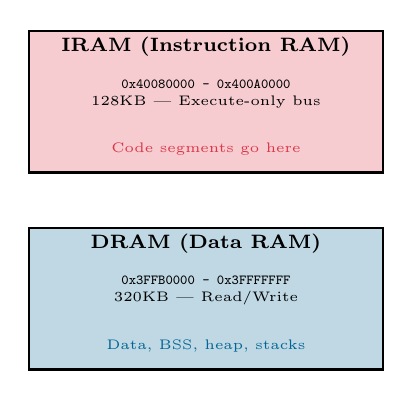
\begin{tikzpicture}
                    % IRAM block
                    \node[layerbox, fill=codered!25, minimum width=4.5cm, minimum height=1.8cm] (iram) at (0,2.5) {};
                    \node[font=\scriptsize\bfseries] at (0,3.2) {IRAM (Instruction RAM)};
                    \node[font=\tiny, align=center] at (0,2.6) {\texttt{0x40080000 - 0x400A0000}\\128KB | Execute-only bus};
                    \node[font=\tiny, text=codered] at (0,1.9) {Code segments go here};
                    
                    % DRAM block  
                    \node[layerbox, fill=espblue!25, minimum width=4.5cm, minimum height=1.8cm] (dram) at (0,0) {};
                    \node[font=\scriptsize\bfseries] at (0,0.7) {DRAM (Data RAM)};
                    \node[font=\tiny, align=center] at (0,0.1) {\texttt{0x3FFB0000 - 0x3FFFFFFF}\\320KB | Read/Write};
                    \node[font=\tiny, text=espblue] at (0,-0.6) {Data, BSS, heap, stacks};
                \end{tikzpicture}
            }
        \end{center}

        \column{0.52\textwidth}
        \begin{block}{The Address Space Problem}
            Linux processes expect fixed virtual addresses (e.g., \texttt{0x8048000}). On ESP32, that address doesn't exist or maps to peripherals.
        \end{block}

        \begin{block}{Solution: Position Independent Code}
            \begin{itemize}
                \item Compile with \texttt{-fPIC -shared}
                \item All references use GOT/relative addressing
                \item Loader performs load-time relocation
                \item Addresses adjusted to actual \texttt{malloc} location
            \end{itemize}
        \end{block}
    \end{columns}
\end{frame}

% ============================================================
% ELF LOADER
% ============================================================
\begin{frame}{ELF Loader: Dynamic Linking on Bare Metal}
    \begin{center}
        \resizebox{0.98\textwidth}{!}{
            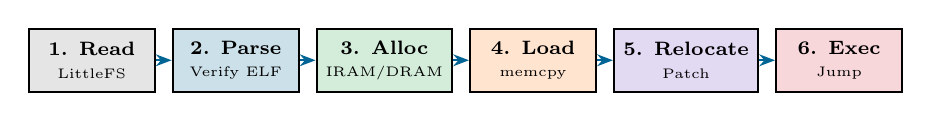
\begin{tikzpicture}[node distance=0.4cm]
                % Pipeline stages
                \node[layerbox, fill=gray!20, minimum width=1.6cm, minimum height=0.8cm] (read) 
                      {\scriptsize\textbf{1. Read}\\\tiny LittleFS};
                \node[layerbox, fill=espblue!20, minimum width=1.6cm, minimum height=0.8cm, right=0.2cm of read] (parse) 
                      {\scriptsize\textbf{2. Parse}\\\tiny Verify ELF};
                \node[layerbox, fill=codegreen!20, minimum width=1.6cm, minimum height=0.8cm, right=0.2cm of parse] (alloc) 
                      {\scriptsize\textbf{3. Alloc}\\\tiny IRAM/DRAM};
                \node[layerbox, fill=codeorange!20, minimum width=1.6cm, minimum height=0.8cm, right=0.2cm of alloc] (load) 
                      {\scriptsize\textbf{4. Load}\\\tiny memcpy};
                \node[layerbox, fill=codepurple!20, minimum width=1.6cm, minimum height=0.8cm, right=0.2cm of load] (reloc) 
                      {\scriptsize\textbf{5. Relocate}\\\tiny Patch};
                \node[layerbox, fill=codered!20, minimum width=1.6cm, minimum height=0.8cm, right=0.2cm of reloc] (exec) 
                      {\scriptsize\textbf{6. Exec}\\\tiny Jump};
                
                \draw[dataarrow] (read) -- (parse);
                \draw[dataarrow] (parse) -- (alloc);
                \draw[dataarrow] (alloc) -- (load);
                \draw[dataarrow] (load) -- (reloc);
                \draw[dataarrow] (reloc) -- (exec);
            \end{tikzpicture}
        }
    \end{center}

    \vspace{0.4cm}
    \begin{columns}[T]
        \column{0.48\textwidth}
        \textbf{Header Validation:}
        \begin{itemize}\setlength{\itemsep}{0pt}
            \item Magic: \texttt{0x7F 'E' 'L' 'F'}
            \item Class: \texttt{ELFCLASS32}, Machine: \texttt{EM\_XTENSA}
            \item Type: \texttt{ET\_DYN} (position independent)
        \end{itemize}
        \footnotesize \textbf{Why ET\_DYN?} Can load at any address.

        \column{0.48\textwidth}
        \textbf{Xtensa Relocations:}
        \begin{itemize}\setlength{\itemsep}{0pt}
            \item \texttt{R\_XTENSA\_RELATIVE}: \texttt{*addr += load\_bias}
            \item \texttt{R\_XTENSA\_SLOT0\_OP}: Patch 18-bit opcode offset
        \end{itemize}
        \footnotesize \textbf{Cache Coherency:} Flush D-Cache, invalidate I-Cache.
    \end{columns}
\end{frame}

% ============================================================
% POSIX SHIM LAYER
% ============================================================
\begin{frame}{POSIX Shim Layer: Syscall Translation}
    \begin{center}
        \resizebox{0.85\textwidth}{!}{
            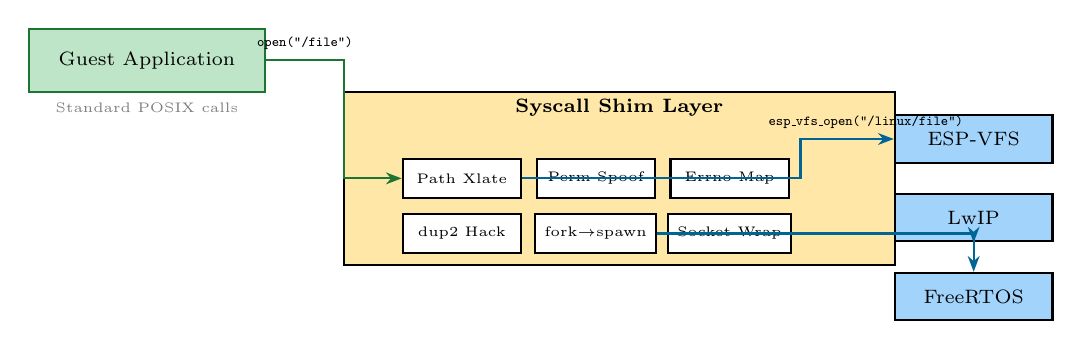
\begin{tikzpicture}
                % Guest app
                \node[guestbox, minimum width=3cm, minimum height=0.8cm] (guest) at (-4.5, 2) {Guest Application};
                \node[font=\tiny, text=gray] at (-4.5, 1.4) {Standard POSIX calls};
                
                % Shim layer detail
                \node[shimbox, minimum width=7cm, minimum height=2.2cm] (shim) at (1.5, 0.5) {};
                \node[font=\scriptsize\bfseries] at (1.5, 1.4) {Syscall Shim Layer};
                
                % Individual shims
                \node[layerbox, fill=white, minimum width=1.5cm, minimum height=0.5cm, font=\tiny] (s1) at (-0.5, 0.5) {Path Xlate};
                \node[layerbox, fill=white, minimum width=1.5cm, minimum height=0.5cm, font=\tiny] (s2) at (1.2, 0.5) {Perm Spoof};
                \node[layerbox, fill=white, minimum width=1.5cm, minimum height=0.5cm, font=\tiny] (s3) at (2.9, 0.5) {Errno Map};
                \node[layerbox, fill=white, minimum width=1.5cm, minimum height=0.5cm, font=\tiny] (s4) at (-0.5, -0.2) {dup2 Hack};
                \node[layerbox, fill=white, minimum width=1.5cm, minimum height=0.5cm, font=\tiny] (s5) at (1.2, -0.2) {fork$\to$spawn};
                \node[layerbox, fill=white, minimum width=1.5cm, minimum height=0.5cm, font=\tiny] (s6) at (2.9, -0.2) {Socket Wrap};
                
                % Host services
                \node[kernelbox, minimum width=2cm, minimum height=0.6cm] (vfs) at (6, 1) {ESP-VFS};
                \node[kernelbox, minimum width=2cm, minimum height=0.6cm] (lwip) at (6, 0) {LwIP};
                \node[kernelbox, minimum width=2cm, minimum height=0.6cm] (rtos) at (6, -1) {FreeRTOS};
                
                % Arrows
                \draw[callarrow] (guest) -- node[above, font=\tiny] {\texttt{open("/file")}} (-2, 2) |- (s1.west);
                \draw[dataarrow] (s1.east) -- (3.8, 0.5) -- (3.8, 1) -- node[above, font=\tiny, pos=0.7] {\texttt{esp\_vfs\_open("/linux/file")}} (vfs);
                \draw[dataarrow] (s6) -| (lwip);
                \draw[dataarrow] (s5) -| (rtos);
            \end{tikzpicture}
        }
    \end{center}

    \vspace{0.3cm}
    \begin{columns}[T]
        \column{0.48\textwidth}
        \begin{block}{Path Translation}
            \begin{itemize}
                \item \texttt{/file} $\to$ \texttt{/linux/file}
                \item \texttt{/dev/*} passed through
                \item Relative paths use task-local CWD
            \end{itemize}
        \end{block}

        \column{0.48\textwidth}
        \begin{block}{Permission Spoofing}
            \begin{itemize}
                \item LittleFS stores no permissions
                \item \texttt{stat()} returns \texttt{st\_mode = 0}
                \item Shim forces \texttt{0777} for compatibility
            \end{itemize}
        \end{block}
    \end{columns}
\end{frame}

% ============================================================
% HARDWARE DRIVER LAYER
% ============================================================
\begin{frame}{Unix-Style Hardware Abstraction: \texttt{/dev/} Drivers}
    \textbf{Design Goal:} Standard POSIX applications control real hardware via familiar \texttt{/dev/} interface.

    \vspace{0.3cm}
    \begin{columns}[T]
        \column{0.48\textwidth}
        \centering
        \resizebox{0.9\textwidth}{!}{
            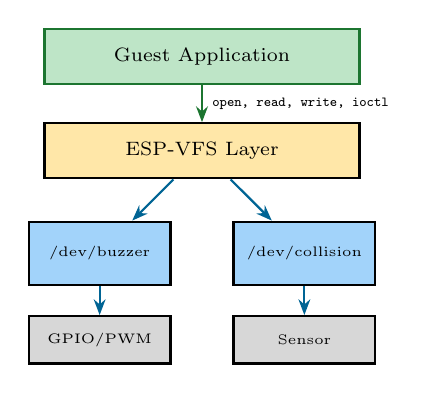
\begin{tikzpicture}
                % Application layer
                \node[guestbox, minimum width=4cm, minimum height=0.7cm] (app) at (0, 4) {Guest Application};
                
                % VFS layer
                \node[shimbox, minimum width=4cm, minimum height=0.7cm] (vfs) at (0, 2.8) {ESP-VFS Layer};
                
                % Device drivers
                \node[kernelbox, minimum width=1.8cm, minimum height=0.8cm] (buzzer) at (-1.3, 1.5) {\tiny /dev/buzzer};
                \node[kernelbox, minimum width=1.8cm, minimum height=0.8cm] (collision) at (1.3, 1.5) {\tiny /dev/collision};
                
                % Hardware
                \node[hwbox, minimum width=1.8cm, minimum height=0.6cm] (gpio) at (-1.3, 0.4) {\tiny GPIO/PWM};
                \node[hwbox, minimum width=1.8cm, minimum height=0.6cm] (sensor) at (1.3, 0.4) {\tiny Sensor};
                
                % Arrows
                \draw[callarrow] (app) -- node[right, font=\tiny] {\texttt{open, read, write, ioctl}} (vfs);
                \draw[dataarrow] (vfs) -- (buzzer);
                \draw[dataarrow] (vfs) -- (collision);
                \draw[dataarrow] (buzzer) -- (gpio);
                \draw[dataarrow] (collision) -- (sensor);
            \end{tikzpicture}
        }

        \column{0.48\textwidth}
        \textbf{Driver Interface:}
        \begin{itemize}\setlength{\itemsep}{0pt}
            \item \texttt{open("/dev/buzzer", O\_RDWR)}
            \item \texttt{write(fd, "1", 1)} --- enable
            \item \texttt{ioctl(fd, SET\_FREQ, 880)}
            \item \texttt{read(fd, buf, len)} --- blocking
        \end{itemize}

        \vspace{0.1cm}
        \textbf{Implementation:}
        \begin{itemize}\setlength{\itemsep}{0pt}
            \item \texttt{esp\_vfs\_register()} registration
            \item FreeRTOS queues for blocking I/O
            \item \texttt{ioctl()} for configuration
        \end{itemize}
    \end{columns}

    \vspace{0.3cm}
    \begin{exampleblock}{Key Benefit}
        \centering
        Unmodified Linux driver patterns work on ESP32.
    \end{exampleblock}
\end{frame}

% ============================================================
% STDOUT REDIRECTION
% ============================================================
\begin{frame}{stdout Redirection: The \texttt{dup2} Challenge}
    \begin{columns}[T]
        \column{0.42\textwidth}
        \textbf{The Problem:}
        \begin{itemize}\setlength{\itemsep}{0pt}
            \item FD 0/1/2 hardwired to UART
            \item \texttt{close(1)} destabilizes logging
            \item Need output over TCP
        \end{itemize}

        \vspace{0.2cm}
        \centering
        \resizebox{0.9\textwidth}{!}{
            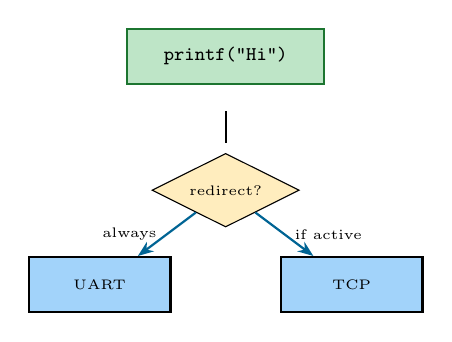
\begin{tikzpicture}
                \node[guestbox, minimum width=2.5cm] (printf) at (0,2.5) {\texttt{printf("Hi")}};
                \draw[thick] (0,1.8) -- (0,1.4);
                \node[draw, diamond, aspect=2, fill=espgold!30, font=\tiny] (check) at (0,0.8) {redirect?};
                \node[kernelbox, minimum width=1.8cm] (uart) at (-1.6,-0.4) {\tiny UART};
                \node[kernelbox, minimum width=1.8cm] (sock) at (1.6,-0.4) {\tiny TCP};
                
                \draw[dataarrow] (check) -- node[left, font=\tiny] {always} (uart);
                \draw[dataarrow] (check) -- node[right, font=\tiny] {if active} (sock);
            \end{tikzpicture}
        }

        \column{0.54\textwidth}
        \begin{block}{Solution: Global State Interceptor}
            \texttt{shim\_dup2(sock, STDOUT)}:
            \begin{itemize}\setlength{\itemsep}{0pt}
                \item Store socket FD in global state
                \item Don't touch VFS table
            \end{itemize}

            \texttt{shim\_write(STDOUT, buf, len)}:
            \begin{itemize}\setlength{\itemsep}{0pt}
                \item Write to UART (debug)
                \item Send to socket (\texttt{MSG\_DONTWAIT})
            \end{itemize}
        \end{block}
        
        \textbf{Result:} Dual-route output.
    \end{columns}
\end{frame}

% ============================================================
% BUILD SYSTEM
% ============================================================
\begin{frame}{Two-Pass Build System: Resolving Circular Dependencies}
    \begin{center}
        \resizebox{0.8\textwidth}{!}{
            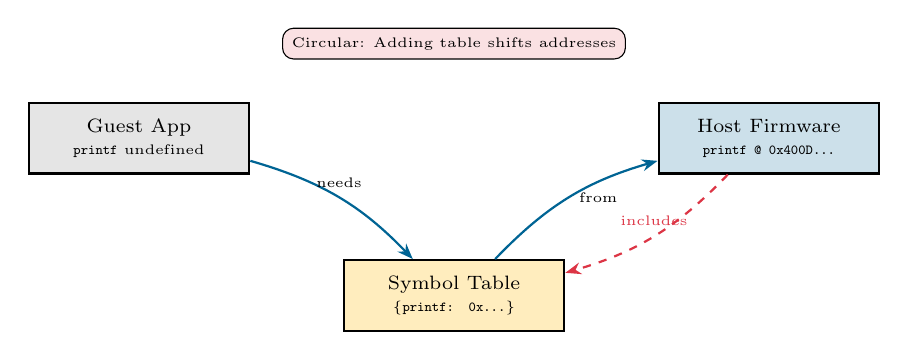
\begin{tikzpicture}
                % The problem visualization
                \node[layerbox, fill=gray!20, minimum width=2.8cm, minimum height=0.9cm] (guest) at (-4, 0) 
                      {\scriptsize Guest App\\\tiny \texttt{printf} undefined};
                \node[layerbox, fill=espblue!20, minimum width=2.8cm, minimum height=0.9cm] (firmware) at (4, 0) 
                      {\scriptsize Host Firmware\\\tiny \texttt{printf @ 0x400D...}};
                \node[layerbox, fill=espgold!30, minimum width=2.8cm, minimum height=0.9cm] (symtab) at (0, -2) 
                      {\scriptsize Symbol Table\\\tiny \texttt{\{printf: 0x...\}}};
                
                \draw[dataarrow, bend left=15] (guest) to node[above, font=\tiny] {needs} (symtab);
                \draw[dataarrow, bend left=15] (symtab) to node[right, font=\tiny] {from} (firmware);
                \draw[dataarrow, bend left=15, codered, dashed] (firmware) to node[above, font=\tiny, text=codered] {includes} (symtab);
                
                \node[draw, fill=codered!15, rounded corners, font=\tiny, align=center] at (0, 1.2) 
                      {Circular: Adding table shifts addresses};
            \end{tikzpicture}
        }
    \end{center}

    \vspace{0.2cm}
    \textbf{Solution: Multi-Stage Pipeline}
    \begin{center}
        \resizebox{0.95\textwidth}{!}{
            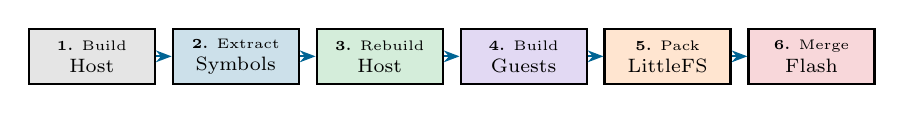
\begin{tikzpicture}[node distance=0.3cm]
                \node[layerbox, fill=gray!20, minimum width=1.6cm, minimum height=0.7cm] (s1) 
                      {\tiny\textbf{1.} Build\\Host};
                \node[layerbox, fill=espblue!20, minimum width=1.6cm, minimum height=0.7cm, right=0.2cm of s1] (s2) 
                      {\tiny\textbf{2.} Extract\\Symbols};
                \node[layerbox, fill=codegreen!20, minimum width=1.6cm, minimum height=0.7cm, right=0.2cm of s2] (s3) 
                      {\tiny\textbf{3.} Rebuild\\Host};
                \node[layerbox, fill=codepurple!20, minimum width=1.6cm, minimum height=0.7cm, right=0.2cm of s3] (s4) 
                      {\tiny\textbf{4.} Build\\Guests};
                \node[layerbox, fill=codeorange!20, minimum width=1.6cm, minimum height=0.7cm, right=0.2cm of s4] (s5) 
                      {\tiny\textbf{5.} Pack\\LittleFS};
                \node[layerbox, fill=codered!20, minimum width=1.6cm, minimum height=0.7cm, right=0.2cm of s5] (s6) 
                      {\tiny\textbf{6.} Merge\\Flash};
                
                \draw[dataarrow] (s1) -- (s2);
                \draw[dataarrow] (s2) -- (s3);
                \draw[dataarrow] (s3) -- (s4);
                \draw[dataarrow] (s4) -- (s5);
                \draw[dataarrow] (s5) -- (s6);
            \end{tikzpicture}
        }
    \end{center}
\end{frame}

% ============================================================
% DEMO 1: V2X COLLISION (Hardware-focused)
% ============================================================
\begin{frame}{Demo 1: V2X Collision Avoidance System}
    \begin{columns}[T]
        \column{0.48\textwidth}
        \begin{center}
            \resizebox{0.4\textwidth}{!}{
                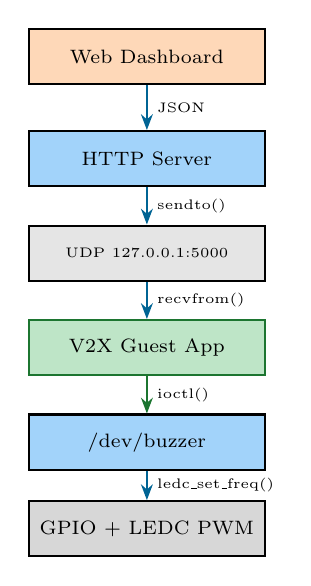
\begin{tikzpicture}
                    % Web UI
                    \node[layerbox, fill=codeorange!30, minimum width=3cm] (web) at (0, 4.5) {Web Dashboard};
                    
                    % HTTP layer
                    \node[kernelbox, minimum width=3cm] (http) at (0, 3.2) {HTTP Server};
                    
                    % UDP loopback
                    \node[layerbox, fill=gray!20, minimum width=3cm] (udp) at (0, 2) {\tiny UDP 127.0.0.1:5000};
                    
                    % Guest app
                    \node[guestbox, minimum width=3cm] (v2x) at (0, 0.8) {V2X Guest App};
                    
                    % Device driver
                    \node[kernelbox, minimum width=3cm] (buzzer) at (0, -0.4) {/dev/buzzer};
                    
                    % Hardware
                    \node[hwbox, minimum width=3cm] (gpio) at (0, -1.5) {GPIO + LEDC PWM};
                    
                    % Arrows with labels
                    \draw[dataarrow] (web) -- node[right, font=\tiny] {JSON} (http);
                    \draw[dataarrow] (http) -- node[right, font=\tiny] {sendto()} (udp);
                    \draw[dataarrow] (udp) -- node[right, font=\tiny] {recvfrom()} (v2x);
                    \draw[callarrow] (v2x) -- node[right, font=\tiny] {ioctl()} (buzzer);
                    \draw[dataarrow] (buzzer) -- node[right, font=\tiny] {ledc\_set\_freq()} (gpio);
                \end{tikzpicture}
            }
        \end{center}

        \column{0.48\textwidth}
        \textbf{Time-to-Collision Calculation:}
        \[
        TTC = \frac{|\vec{P}_{target} - \vec{P}_{ego}|}{|\vec{V}_{target} - \vec{V}_{ego}|}
        \]

        \begin{block}{Application Logic}
            Open device: \texttt{open("/dev/buzzer", O\_RDWR)}

            If collision imminent:
            \begin{itemize}
                \item Set frequency: \texttt{ioctl(fd, SET\_FREQ, 880)}
                \item Enable alarm: \texttt{write(fd, "1", 1)}
            \end{itemize}
        \end{block}
    \end{columns}
\end{frame}
% ============================================================
% DEMO 2: COMMAND & CONTROL
% ============================================================
\begin{frame}{Demo 2: Distributed Command \& Control}
    \begin{columns}[T]
        \column{0.46\textwidth}
        \begin{center}
            \resizebox{0.9\textwidth}{!}{
                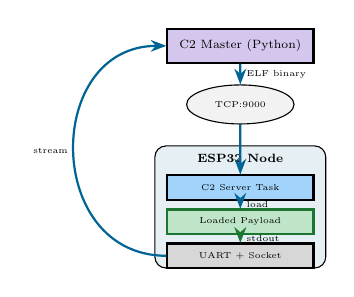
\begin{tikzpicture}[scale=0.62, transform shape]
                    % Master
                    \node[layerbox, fill=codepurple!30, minimum width=3cm] (master) at (0, 4) {C2 Master (Python)};
                    
                    % Network cloud
                    \node[draw, ellipse, fill=gray!10, minimum width=2.2cm, minimum height=0.8cm, font=\tiny] (net) at (0, 2.8) {TCP:9000};
                    
                    % ESP32 box
                    \node[draw, fill=espblue!10, minimum width=3.5cm, minimum height=2.5cm, rounded corners] (esp) at (0, 0.7) {};
                    \node[font=\scriptsize\bfseries] at (0, 1.7) {ESP32 Node};
                    \node[kernelbox, minimum width=3cm, minimum height=0.5cm] (c2srv) at (0, 1.1) {\tiny C2 Server Task};
                    \node[guestbox, minimum width=3cm, minimum height=0.5cm] (payload) at (0, 0.4) {\tiny Loaded Payload};
                    \node[hwbox, minimum width=3cm, minimum height=0.5cm] (uart) at (0, -0.3) {\tiny UART + Socket};
                    
                    % Data flow
                    \draw[dataarrow] (master) -- node[right, font=\tiny] {ELF binary} (net);
                    \draw[dataarrow] (net) -- (c2srv);
                    \draw[dataarrow] (c2srv) -- node[right, font=\tiny] {load} (payload);
                    \draw[callarrow] (payload) -- node[right, font=\tiny] {stdout} (uart);
                    
                    % FIXED ARROW: Uses out/in=180 to arc explicitly around the left side
                    \draw[dataarrow] (uart.west) to[out=180, in=180, looseness=1.5] node[left, font=\tiny] {stream} (master.west);
                \end{tikzpicture}
            }
        \end{center}

        \column{0.5\textwidth}
        \textbf{Protocol:}
        \begin{enumerate}
            \item Master sends: 4-byte magic + 4-byte size + ELF
            \item ESP32 writes to \texttt{/linux/payload.elf}
            \item Loader parses, allocates, relocates, executes
            \item stdout streams back over same connection
        \end{enumerate}

        \begin{alertblock}{Advantage}
            Update 4KB application vs. reflash 4MB firmware.\\
            50 drones: 100+ min $\to$ seconds.
        \end{alertblock}
    \end{columns}
\end{frame}

% ============================================================
% SECURITY & LIMITATIONS
% ============================================================
\begin{frame}{Security Model \& Limitations}
    \begin{columns}[T]
        \column{0.48\textwidth}
        \begin{block}{Library OS Risks}
            \begin{itemize}
                \item \textbf{No memory isolation:} Guest can access any physical address
                \item \textbf{No fault isolation:} Guest crash $\to$ full chip reboot
                \item \textbf{Shared address space:} Guests can interfere with each other
            \end{itemize}
        \end{block}

        \column{0.48\textwidth}
        \textbf{Resource Constraints:}
        \begin{table}
        \begin{tabular}{lr}
        \toprule
        \textbf{Resource} & \textbf{Limit} \\
        \midrule
        Total DRAM & 320KB \\
        Available for guests & $\sim$100KB \\
        Task stack (min) & 4KB \\
        Max concurrent guests & $\sim$15 \\
        Guest IRAM & $\sim$32KB \\
        \bottomrule
        \end{tabular}
        \end{table}
    \end{columns}

    \vspace{0.3cm}
    \begin{alertblock}{Threat Model}
        \centering
        Trusted guest code in controlled deployments. Not suitable for public app stores.
    \end{alertblock}
\end{frame}

% ============================================================
% CONTRIBUTIONS & FUTURE WORK
% ============================================================
\begin{frame}{Contributions \& Future Directions}
    \begin{columns}[T]
        \column{0.48\textwidth}
        \textbf{Key Contributions:}
        \begin{enumerate}
            \item \textbf{Dynamic ELF Loading}
                \begin{itemize}
                    \item Full Xtensa relocation support
                    \item IRAM/DRAM split allocation
                \end{itemize}
            \item \textbf{POSIX Compatibility Layer}
                \begin{itemize}
                    \item File I/O with path translation
                    \item BSD sockets via LwIP
                \end{itemize}
            \item \textbf{Unix-style Driver Model}
                \begin{itemize}
                    \item \texttt{/dev/} nodes for hardware
                    \item \texttt{ioctl()} configuration
                \end{itemize}
        \end{enumerate}

        \column{0.48\textwidth}
        \textbf{Future Directions:}
        \begin{itemize}
            \item \textbf{Short term:}
                \begin{itemize}
                    \item Shared libraries (\texttt{libc.so})
                    \item Multi-core pinning
                \end{itemize}
            \item \textbf{Long term:}
                \begin{itemize}
                    \item MicroPython/Lua as guests
                    \item WASM for sandboxed execution
                    \item ESP32-S3 PMS integration
                \end{itemize}
        \end{itemize}
    \end{columns}

    \vspace{0.2cm}
    \begin{exampleblock}{Vision}
        \centering
        A microcontroller that behaves like a tiny Linux box ---\\
        dynamic, network-programmable, yet real-time.
    \end{exampleblock}
\end{frame}

\end{document}